\documentclass{beamer}
\usepackage{dsfont}
\usetheme{CambridgeUS}
%\usecolortheme{lily}
\mode<presentation>
\title[Logic, Computability, $\mathds{N}$]{Exploring Logic \& Computability via the Natural Numbers}
\institute[NIC]{Near Infinity Corporation}
\author[Ed MacDonald]{Ed MacDonald \\ \texttt{emacdona@nearinfinity.com}}
%\date[ISPN ’80]{27th International Symposium of Prime Numbers}
\begin{document}

\begin{frame}
\titlepage
\end{frame}

\begin{frame}
   \frametitle{What is true of these two pictures??}
   \begin{columns}
      \begin{column}{5cm}
         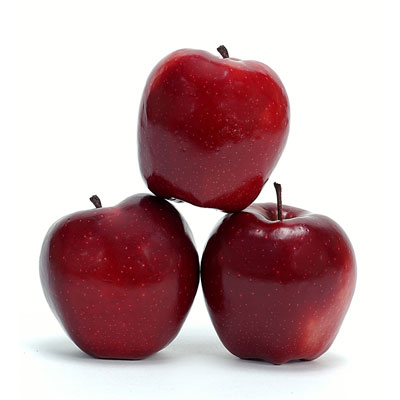
\includegraphics[width=4cm,height=4cm]{images/apples.jpg}
      \end{column}
      \begin{column}{5cm}
         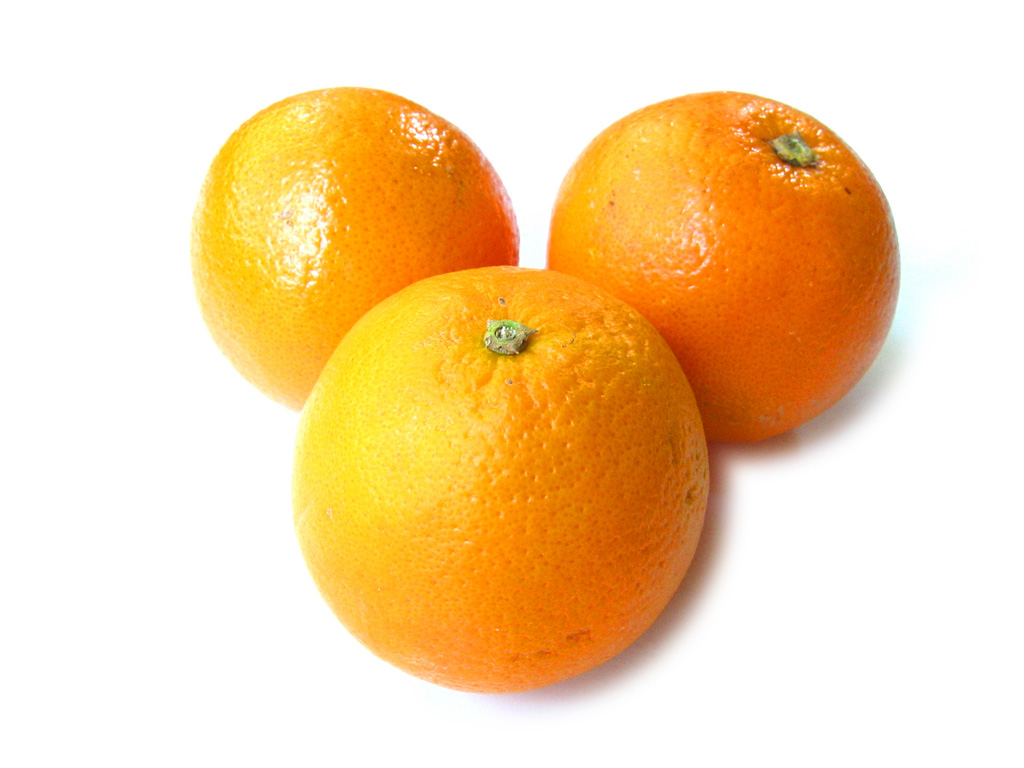
\includegraphics[width=4cm,height=3cm]{images/oranges.jpg}
      \end{column}
   \end{columns}
\end{frame}

\begin{frame}
   \frametitle{What is a Natural Number?}
   1858: Giuseppe Peano born\\
\end{frame}

\begin{frame}
\end{frame}

\end{document}

